%%%%%%%%%%%%%%%%%%%%%%%%%%%%%%%%%%%%%%%%%
% a0poster Portrait Poster
% LaTeX Template
% Version 1.0 (22/06/13)
%
% The a0poster class was created by:
% Gerlinde Kettl and Matthias Weiser (tex@kettl.de)
% 
% This template has been downloaded from:
% http://www.LaTeXTemplates.com
%
% License:
% CC BY-NC-SA 3.0 (http://creativecommons.org/licenses/by-nc-sa/3.0/)
%
%%%%%%%%%%%%%%%%%%%%%%%%%%%%%%%%%%%%%%%%%

%----------------------------------------------------------------------------------------
%	PACKAGES AND OTHER DOCUMENT CONFIGURATIONS
%----------------------------------------------------------------------------------------

\documentclass{a0poster}
\usepackage[pass,paperwidth=34in,paperheight=22in]{geometry}

\usepackage{multicol} % This is so we can have multiple columns of text side-by-side
\columnsep=100pt % This is the amount of white space between the columns in the poster
\columnseprule=3pt % This is the thickness of the black line between the columns in the poster

\usepackage[svgnames]{xcolor} % Specify colors by their 'svgnames'

\usepackage{graphicx} % Required for including images
\usepackage{booktabs} % Top and bottom rules for table
\usepackage{mathdots}
\usepackage[font=small,labelfont=bf]{caption} % Required for specifying captions to tables and figures
\usepackage{amsfonts, amsmath, amsthm, amssymb} % For math fonts, symbols and environments
\usepackage{wrapfig} % Allows wrapping text around tables and figures
\makeatletter
\renewenvironment{abstract}{%
    \if@twocolumn
      \section*{\abstractname}%
    \else %% <- here I've removed \small
      \begin{center}%
        {\bfseries \LARGE\abstractname\vspace{\z@}}%  %% <- here I've added \Large
      \end{center}%
      \quotation
    \fi}
    {\if@twocolumn\else\endquotation\fi}
\makeatother

\usepackage{sectsty}
\sectionfont{\fontsize{60}{65}\selectfont}
\subsectionfont{\fontsize{50}{60}\selectfont}

\begin{document}

%----------------------------------------------------------------------------------------
%	POSTER HEADER 
%----------------------------------------------------------------------------------------

% The header is divided into two boxes:
% The first is 75% wide and houses the title, subtitle, names, university/organization and contact information
% The second is 25% wide and houses a logo for your university/organization or a photo of you
% The widths of these boxes can be easily edited to accommodate your content as you see fit


\begin{minipage}[c]{\linewidth}
\begin{centering}
\veryHuge \color{NavyBlue} \textbf{Data Driven Reduced Order Modeling} \color{Black}\\[1cm] % Title
%\Huge\textit{Subtitle}\\[2cm] % Subtitle
\Huge Aryn Harmon$^1$ and Jason Turner$^2$\\
\huge University of Illinois at Urbana-Champaign, Champaign, Illinois, U.S.A.\\[0.4cm] % University/organization
\Large $^1$ \texttt{arynh2@illinois.edu}, $^2$ \texttt{jasonet2@illinois.edu}\\
\end{centering}
\end{minipage}

\vspace{1cm} % A bit of extra whitespace between the header and poster content

%----------------------------------------------------------------------------------------

\begin{multicols}{3} % This is how many columns your poster will be broken into, a portrait poster is generally split into 2 columns

%----------------------------------------------------------------------------------------
%	ABSTRACT
%----------------------------------------------------------------------------------------

\color{Navy} % Navy color for the abstract

\hrulefill
\vspace{0.5cm}
\begin{abstract}
\LARGE

\textsc{Model Order Reduction} (MOR) can be applied to many-dimensional problems to reduce the computational cost of finding solutions. We created a high fidelity model for the linear convection and diffusion equation using finite difference methods. Using data from this model, we successfully constructed an accurate lower order model using proper orthogonal decomposition.

\end{abstract}
\hrulefill

%----------------------------------------------------------------------------------------
%	OBJECTIVES
%----------------------------------------------------------------------------------------

\color{Black} % DarkSlateGray color for the rest of the content

\section{Main Objectives}
\huge
\begin{enumerate}
\item Make online computation possible in computationally challenging problems.
\item Speed up analysis of problems with many degrees of freedom.
\item Produce an understanding of physical processes which are currently obscured by complexity.
\end{enumerate}

%----------------------------------------------------------------------------------------
%	INTRODUCTION
%----------------------------------------------------------------------------------------

\color{Black} % SaddleBrown color for the introduction

\section{Introduction}
\LARGE
\begin{itemize}
  \item Linear Convection and Diffusion Equation describes movement and diffusion of a wave in one dimension.
  $$\frac{\partial u}{\partial t} + c \frac{\partial u}{\partial x} = \frac{1}{\mathrm{Re}} \frac{\partial^2 u}{\partial x^2}$$
  $$\vec{u}^{\,n+1} = \mathcal{L}(\vec{u}^{\,n}) = \mathrm{\textbf{B}} \vec{u}^{\,n}$$
  \item Black-Scholes Model prices European options.
  $$\frac{\partial w}{\partial t} = rw - rx \frac{\partial w}{\partial x} - \frac{1}{2} v^2 x^2 \frac{\partial^2 w}{\partial x^2}$$
  \item Viscous Burger's Equation (short description, mention nonlinearity)
  $$\frac{\partial u}{\partial t} + u \frac{\partial u}{\partial x} = \nu \frac{\partial^2 u}{\partial x^2}$$
  $$\mathrm{\textbf{J}} \left( u^{n+1} - u^n \right) - \mathrm{\textbf{R}} \left( u^n \right)=0 \implies u^{n+1} = \mathcal{L}(\vec{u}^{\,n}) + \mathcal{N}(\vec{u}^{\,n})$$
  \item MOR uses symmetries in problems to find answers faster.
\end{itemize}

%----------------------------------------------------------------------------------------
%	MATERIALS AND METHODS
%----------------------------------------------------------------------------------------

\section{Methods}
\LARGE
%---------------------------------------------------
\subsection{Full Order Model}

Finite Difference Scheme:
$$\frac{\partial u}{\partial x} = \frac{u_{i+1} - u_{i-1}}{2 \Delta x} + \mathcal{O}(\Delta x^2)$$
$$\frac{\partial^2 u}{\partial x^2} = \frac{u_{i+1} - 2u_i + u_{i-1}}{\Delta x^2} + \mathcal{O}(\Delta x^2)$$
$$\vdots$$
$$\frac{\partial \vec{u}_i}{\partial t} = \left(\frac{1}{\mathrm{Re} \Delta x^2} - \frac{c}{2 \Delta x}\right)u_{i+1} - \frac{2}{\Delta x^2} u_i + \left( \frac{1}{\mathrm{Re} \Delta x^2} + \frac{c}{2 \Delta x} \right) u_{i-1}$$

\subsection{Reduced Order Model}

The goal of MOR is to lower the rank needed to evolve a system to solve it; this can be done with \textbf{singular value decomposition}.
$$\mathrm{min} \{ ||\textbf{X} - u \cdot v||_F \} \implies A = U \Sigma V^T$$
The number of modes we use to create the model is dependent on how many singular values are used. In the case of linear convection and diffusion, we used three modes to model with nearly no error.

%----------------------------------------------------------------------------------------
%	RESULTS 
%----------------------------------------------------------------------------------------

\section{Results}



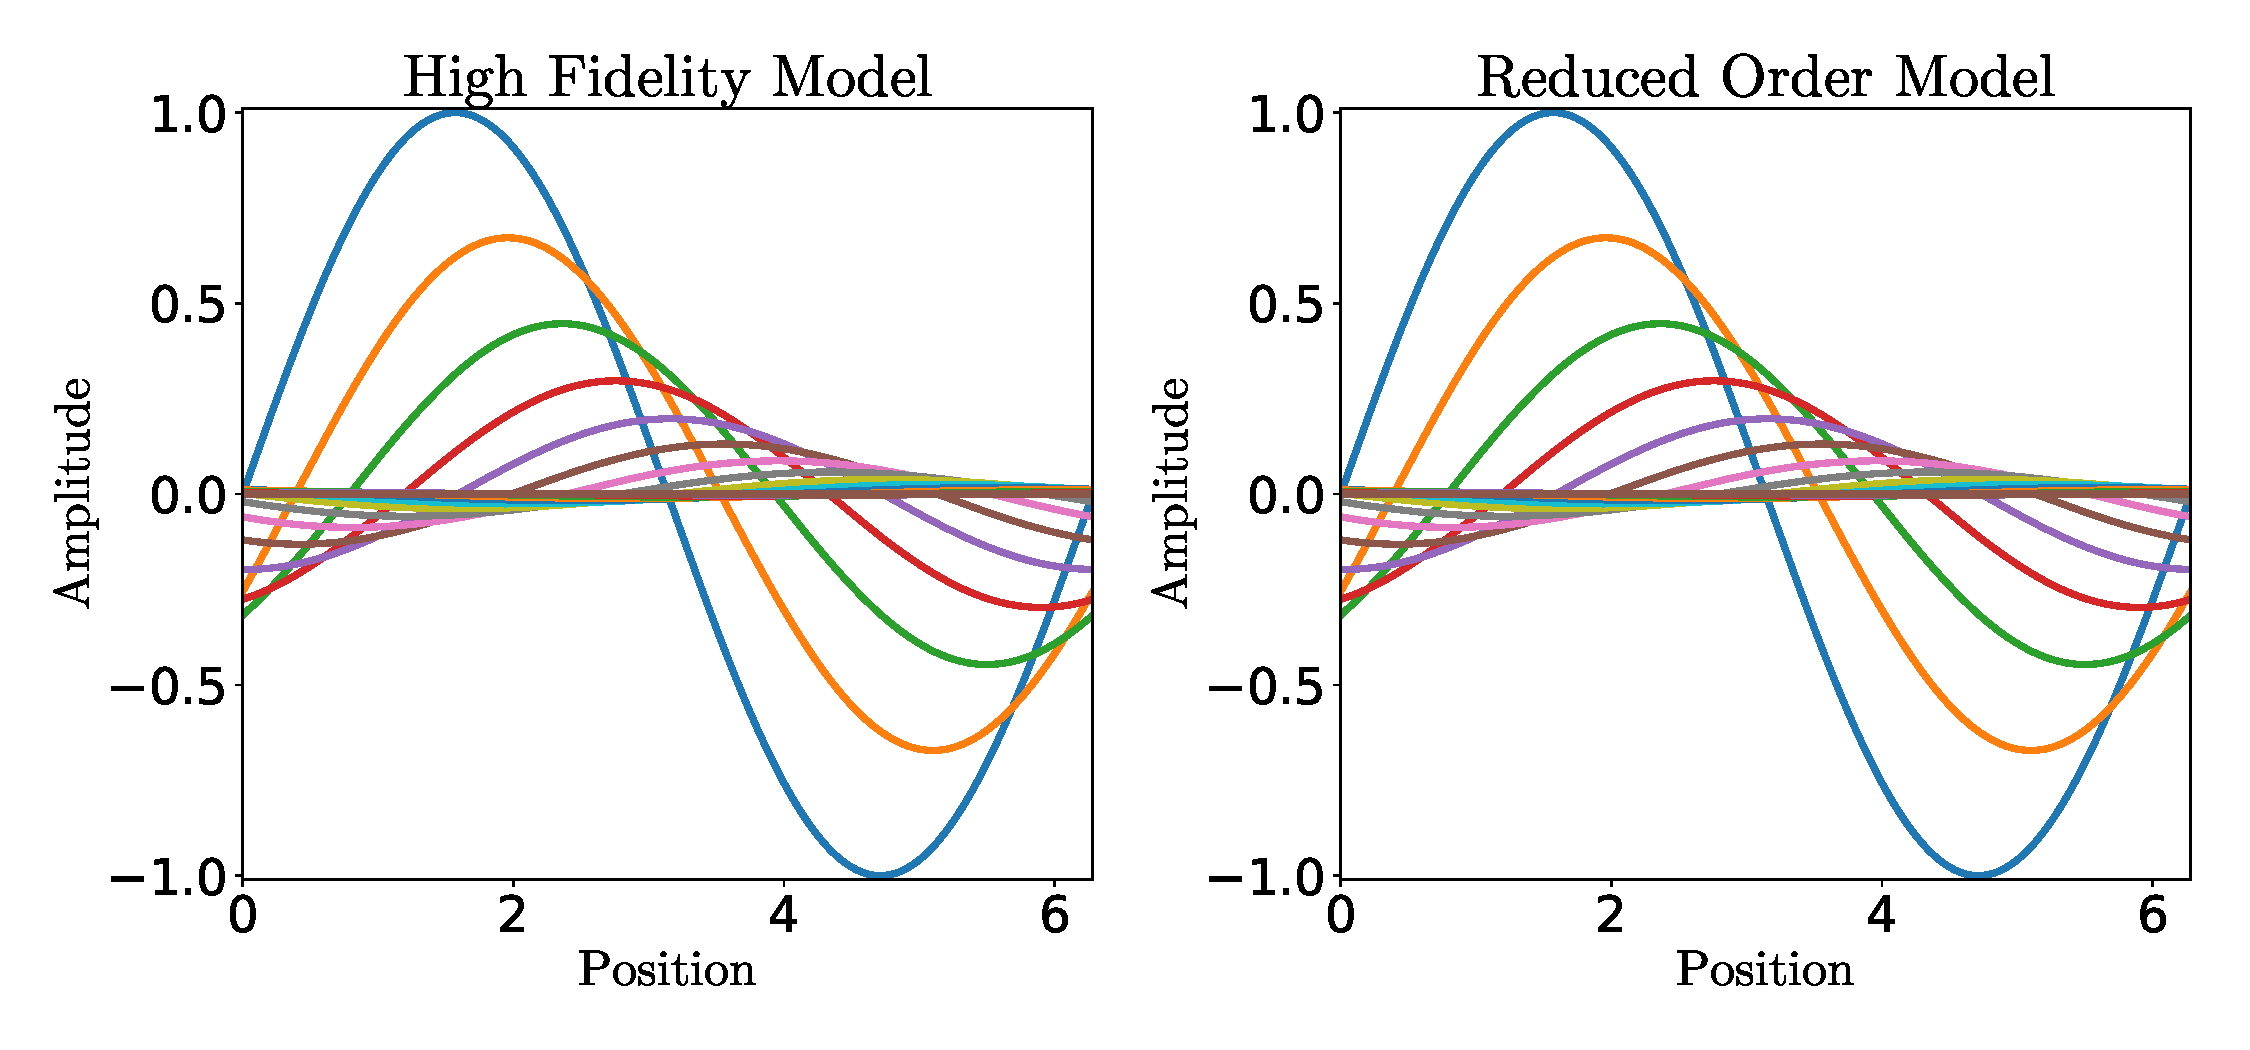
\includegraphics[width=\linewidth]{fig.pdf}

%----------------------------------------------------------------------------------------
%	CONCLUSIONS
%----------------------------------------------------------------------------------------

\color{Navy} % SaddleBrown color for the conclusions to make them stand out

\section{Conclusions}

\begin{itemize}
\item 
\end{itemize}

\color{DarkSlateGray} % Set the color back to DarkSlateGray for the rest of the content

%----------------------------------------------------------------------------------------
%	FORTHCOMING RESEARCH
%----------------------------------------------------------------------------------------

\section{Forthcoming Research}



%----------------------------------------------------------------------------------------
%	REFERENCES
%----------------------------------------------------------------------------------------

\nocite{*} % Print all references regardless of whether they were cited in the poster or not
\bibliographystyle{plain} % Plain referencing style
\bibliography{sample} % Use the example bibliography file sample.bib

%----------------------------------------------------------------------------------------
%	ACKNOWLEDGEMENTS
%----------------------------------------------------------------------------------------

\section{Acknowledgements}

\begin{minipage}[c]{0.5\linewidth}
\begin{centering}

\includegraphics[width=\linewidth]{pure_logof.pdf}
\end{centering}
\end{minipage}
\begin{minipage}[c]{0.5\linewidth}
\begin{centering}

\includegraphics[width=\linewidth]{logo.jpg}
\end{centering}
\end{minipage}
%----------------------------------------------------------------------------------------

\end{multicols}
\end{document}